\section{Square coverings for affine motion}\label{b:linear-coverings}

We first cover the whole transverse plane for a frozen affine velocity
field. The squares keep their side lengths and orientations; only their
centers move. An inverse estimate will then locate the centers needed
near a compact set of labels. Neither step requires a smallness bound on the
individual shear coefficients.

\begin{lemma}[A deformed square grid]\label{b:lattice}
Let $\alpha,\beta\in\R$ satisfy $0\le\alpha\beta<1$.
The closed unit squares with centers
\[
 (i+\alpha j,\,\beta i+j),\qquad (i,j)\in\Z^2,
\]
cover $\R^2$.
\end{lemma}
\begin{proof}
Write $R(t)=\lfloor t+1/2\rfloor$. For a target $u=(u_1,u_2)$,
it suffices to find integers satisfying
\[
 i=R(u_1-\alpha j),\qquad j=R(u_2-\beta i).
\]
Consider $F(i)=R(u_1-\alpha R(u_2-\beta i))$. If
$\alpha\beta>0$, the two multiplications either both preserve or
both reverse order, so $F$ is nondecreasing. If either coefficient
is zero, $F$ is constant and hence still nondecreasing. Moreover,
\[
 F(i)=\alpha\beta i+O(1)\qquad(|i|\to\infty).
\]
Since $\alpha\beta<1$, there are integers $i_-<i_+$ with
$F(i_-)\ge i_-$ and $F(i_+)\le i_+$. Monotonicity makes the
finite integer interval between them invariant. Iteration from $i_-$
is nondecreasing and bounded, so it reaches a fixed point. Setting
$j=R(u_2-\beta i)$ gives the required pair. Each coordinate error
is at most $1/2$, including equality at the square boundaries.
\end{proof}

This iteration is a finite-chain instance of Tarski's monotone
fixed-point principle \cite[Theorem~1]{Tarski1955}. The positive-product
covering also follows from the signed tiling identity of Kolountzakis
\cite[Section~2.3, equations~(17)--(20)]{Kolountzakis1998}.
After taking its parameters to be $|\alpha|,|\beta|$ and reflecting
one coordinate when necessary, that identity gives the lattice sum of
a unit-square indicator minus a rectangle indicator as $1$ almost
everywhere. The rectangle contribution is nonnegative, so the squares
cover almost everywhere. Their closed, locally finite union then
covers every point. When both parameters have absolute value below
one, Stein's notched-square construction already supplies this
covering \cite[Theorem~7 and equations~(13)--(14)]{Kolountzakis1998}.
The direct proof above includes the zero-product cases as well.

\begin{lemma}[An orthogonal zero-diagonal basis]\label{b:zero-diagonal}
Let $A$ be a real $2\times2$ matrix with $\tr A=0$.
There is an orthonormal basis in which
\[
 A=\begin{pmatrix}0&b\\c&0\end{pmatrix},\qquad bc=-\det A.
\]
\end{lemma}
\begin{proof}
For a unit vector $e$, let $e^\perp$ be its counterclockwise
quarter-turn and put $q(e)=e^{\mathsf T}Ae$. The trace identity
gives $q(e)+q(e^\perp)=0$. Continuity on the quarter-circle
between these vectors supplies a unit vector with $q(e)=0$.
Then $q(e^\perp)=0$ also. The determinant gives the formula for
the product of the off-diagonal entries.
\end{proof}

\begin{lemma}[Affine square covering and center control]\label{b:affine-cover}
Let $L>0$ and let $A$ be a real $2\times2$ matrix satisfying
\[
 \tr A=0,\qquad -L^{-2}<\det A\le0.
\]
Fix $p_0,v_0\in\R^2$ and write $W(p)=v_0+A(p-p_0)$.
There is an orthonormal basis $e_1,e_2$ such that, for every
$\tau>0$, the lattice
\[
 \Lambda=p_0+\tau\Z e_1+\tau\Z e_2
\]
and its closed squares
\[
 T_l=l+[-\tau/2,\tau/2]e_1+[-\tau/2,\tau/2]e_2
 \qquad(l\in\Lambda)
\]
satisfy
\[
 \R^2=\bigcup_{l\in\Lambda}\bigl(T_l+sW(l)\bigr)
 \qquad(|s|\le L).
\]
If $x$ belongs to the translated tile indexed by $l$, then
$|x-l-sW(l)|\le\tau$. Furthermore,
\begin{equation}\label{b:affine-inverse}
 \|(I+sA)^{-1}\|
 \le \frac{1+L\|A\|}{1+L^2\det A}
 \qquad(|s|\le L),
\end{equation}
where the norm is the Euclidean operator norm.
\end{lemma}
\begin{proof}
Choose the basis from Lemma~\ref{b:zero-diagonal}. After subtracting
$p_0+sv_0$ and using this basis in units of $\tau$, the centers are
\[
 (i+sbj,\,sci+j).
\]
Their two parameters have product $s^2bc=-s^2\det A\in[0,1)$,
so Lemma~\ref{b:lattice} applies. The distance from a point of a
square to its center is at most $\tau/\sqrt2$, giving the stated
bound. Cayley--Hamilton and $\tr A=0$ give
\[
 A^2=-(\det A)I,\qquad
 (I+sA)^{-1}=\frac{I-sA}{1+s^2\det A}.
\]
The denominator is at least $1+L^2\det A>0$, which proves
\eqref{b:affine-inverse}.
\end{proof}

Figure~\ref{b:figure-lattice} shows the case of equal positive
off-diagonal parameters. In the affine covering, the tiles keep their
area even though the center map has determinant
$1+s^2\det A\le1$.

\begin{figure}[tb]
\centering
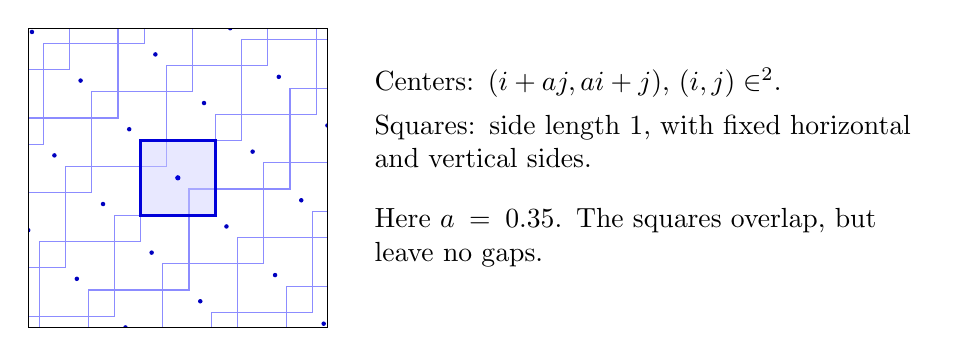
\begin{tikzpicture}[scale=0.95]
 \begin{scope}
  \clip (-2,-2) rectangle (2,2);
  \foreach \i in {-4,...,4} {\foreach \j in {-4,...,4} {
   \pgfmathsetmacro{\cx}{\i+.35*\j}
   \pgfmathsetmacro{\cy}{\j+.35*\i}
   \draw[blue!45,line width=.4pt]
     ({\cx-.5},{\cy-.5}) rectangle ({\cx+.5},{\cy+.5});
   \fill[blue!75!black] (\cx,\cy) circle (.03);
  }}
  \fill[blue!20,opacity=.45] (-.5,-.5) rectangle (.5,.5);
  \draw[blue!85!black,line width=1.1pt] (-.5,-.5) rectangle (.5,.5);
  \fill[blue!85!black] (0,0) circle (.035);
 \end{scope}
 \draw (-2,-2) rectangle (2,2);
 \node[align=left,anchor=west,text width=7cm] at (2.5,.8)
   {Centers: $(i+aj,ai+j)$, $(i,j)\in\Z^2$.\\[4pt]
    Squares: side length $1$, with fixed horizontal and vertical sides.};
 \node[align=left,anchor=west,text width=7cm] at (2.5,-.8)
   {Here $a=0.35$. The squares overlap, but leave no gaps.};
\end{tikzpicture}
\caption{A bounded window in the lattice covering of
Lemma~\ref{b:lattice}, with the square at the origin highlighted.
The squares keep their original shape and orientation as their centers move.
The affine construction uses an orthonormal basis for each frozen
differential. Its finite approximation retains fine-grid centers only
near the corresponding coarse label square.}
\label{b:figure-lattice}
\end{figure}


The square-zero case has a particularly simple interpretation. If
$A\ne0$ and $A^2=0$, then $\operatorname{im}A=\ker A$ is a line.
Choose $e_1$ along that line. In an orthonormal basis the map is
$(x,y)\mapsto(dy,0)$ for some $d\in\R$. After removing the common
translation, row $j$ of the square lattice moves horizontally by
$sd\tau j$. Its vertical interval stays fixed, and the horizontal
intervals in each row still cover the line. Thus the squares cover
for every $s\in\R$ and every $d$, as illustrated in
Figure~\ref{b:figure-rows}. For $A=0$ this is the ordinary square
grid. This explains directly why no bound on the shear is needed
in the square-zero case.

\begin{figure}[ht]
\centering
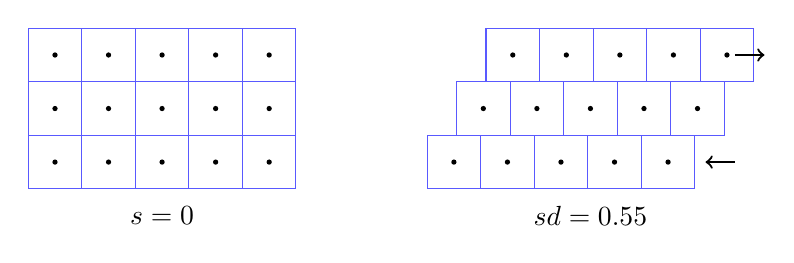
\begin{tikzpicture}[scale=.68]
 \begin{scope}
  \foreach \j in {-1,0,1} {
   \foreach \i in {-2,-1,0,1,2} {
    \draw[blue!65] (\i-.5,\j-.5) rectangle (\i+.5,\j+.5);
    \fill (\i,\j) circle (1.4pt);
   }
  }
  \node at (0,-2.0) {$s=0$};
 \end{scope}
 \begin{scope}[xshift=8cm]
  \foreach \j in {-1,0,1} {
   \foreach \i in {-2,-1,0,1,2} {
    \draw[blue!65] (\i+.55*\j-.5,\j-.5) rectangle (\i+.55*\j+.5,\j+.5);
    \fill (\i+.55*\j,\j) circle (1.4pt);
   }
  }
  \draw[->,thick] (2.7,1) -- (3.25,1);
  \draw[->,thick] (2.7,-1) -- (2.15,-1);
  \node at (0,-2.0) {$sd=0.55$};
 \end{scope}
\end{tikzpicture}
\caption{Sliding rows with $\tau=1$, after removing the common
translation. The tiles remain squares while row $j$ moves horizontally
by $sdj$. Each drawing shows a finite portion of a grid extending
infinitely in both directions. No gaps arise between the closed rows.}
\label{b:figure-rows}
\end{figure}

